\subsection{TOHTN Formalism}
\label{prelim: formalism}
In this section we first define what HTN and TOHTN problems are from a formal perspective \ref{prelim: tohtn problems}. Afterwards we take a short look at the algorithmic worst case complexity of HTN and TOHTN planning \ref{prelim: tohtn complexity}. We conclude by taking a short look at how hierarchical and classical planning compare in \ref{prelim: planning differences} and present the way in which we visualize hierarchical problems in this work in \ref{prelim: graphic tohtn}.

\subsubsection{Defining TOHTN Planning Problems}
\label{prelim: tohtn problems}
Both HTN and TOHTN planning are based of decomposing a list of initial tasks down into smaller subtasks until those subtasks can be achieved by simple actions. A number of formalisms for HTN plannings exist \cite{georgievski2015htn, behnke2018tracking, schreiber2021lilotane}. These formalisms are similar but differ slightly to suit specific planning approaches. In this work, we will reuse the formalism we introduced in \cite{bretl2021parallel} which is built on the definition by \cite{georgievski2015htn}.

\begin{definition} % predicate
	A \textbf{predicate} consists of two parts. Firstly a predicate symbol $p \in \mathcal{P}$ where $\mathcal{P}$ is the finite set of predicate symbols. Secondly of a list of terms $\tau_1, \ldots, \tau_k$ where each term $\tau_i$ is either a constant symbol $c \in \mathcal{C}$, with $\mathcal{C}$ being the finite set of constant symbols, or a variable symbol $v \in \mathcal{V}$, where $\mathcal{V}$ is the infinite set of variable symbols. \\
	The set of all predicates is called $\mathcal{Q}$.
\end{definition}
With the definition of a predicate in place, we can then define a grounding as well as our world state.
\begin{definition} % grounding
	A \textbf{ground predicate} is a predicate where the terms contain no variable symbols or, in other words, a predicate that contains only constant symbols.
\end{definition}
\begin{definition} % state
	A \textbf{state} $s \in 2^{\mathcal{Q}}$ is a set of ground predicates for which we make the closed-world-assumption. Under the closed-world-assumption, only positive predicates are explicitly represented in $s$. All predicates not in $s$ are implicitly negative.
\end{definition}

\begin{definition} % primitive task/ action
	With $T_p$ the set of primitive task symbols, a \textbf{primitive task} $t_p$ is defined as a triple $t_p(\Tilde{t}_p (a_1, \ldots, a_k), pre(t_p), eff(t_p))$. $\Tilde{p} \in T_p$ is the task symbol, $a_1, \ldots, a_k \in \mathcal{C} \cup \mathcal{V}$ are the task arguments, $pre(t_p) \in 2^{\mathcal{P}}$ the preconditions and $eff(t_p) \in 2^{\mathcal{P}}$ the effects of the primitive task $t_p$. We further define the positive and negative preconditions of $t_p$ as $pre^+(t_p) := \{p \in pre(t_p) : p \text{ is positive}\}$ and $pre^-(t_p) := \{p \in pre(t_p) : p \text{ is negative}\}$. We define $eff^+(t_p)$ and $eff^-(t_p)$ analogously. \\
	We call a fully ground primitive task an \textbf{action}.
\end{definition}

As preconditions and effects may not be concerned with the whole world state the closed-world assumption does not apply to them. To any HTN instance we could create an equivalent one where each precondition and effect cares about the whole world state. This would be achieved by instantiating all the "don't care" terms in preconditions and effects with all possible combinations of predicates. Doing this would, however, come at the price of a huge blowup of our planning problem. \\

\begin{definition} % applicable, application
	An action $t_p$ is \textbf{applicable} in state $s$ if $pre^+(t_p) \subseteq s$ and $pre^-(t_p) \cap s = \emptyset$. The \textbf{application} of $t_p$ in state $s$ results in the new state $s' = (s \setminus eff^-(t_p)) \cup eff^+(t_p)$.
\end{definition}

\begin{definition} % compound task/ abstract task
	We define a \textbf{compound task} as $t_c = \Tilde{t}_c(a_1, \ldots, a_k)$, where $\Tilde{t_c} \in T_c$ is the task symbol from the finite set of compound task symbols $T_c$ and $a_1, \ldots, a_k$ are the task arguments.
\end{definition}
Primitive and compound tasks together form task networks. In places where both can be used, we will refer to them simply as tasks $t \in T$.

\begin{definition} % task network
	Let $T = T_p \bigcup T_c$ be a set of primitive and compound tasks. A task network is a tuple $\tau = (T, \psi)$ consisting of tasks $T$ and constraints $\psi$ between those tasks.
\end{definition}

\begin{definition} % method, reduction
	Let $M$ be a finite set of method symbols and $T = T_p \bigcup T_c$ a set of primitive and compound tasks. A \textbf{method} $m = (\Tilde{m}(a_1, \ldots, a_k), t_c, pre(m), subtasks(m), constraints(m))$ is a tuple consisting of the method symbol $\Tilde{m}$, the method arguments $a_1, \ldots, a_k$, the associated compound task $t_c \in T_c$ the method refers to, a set of preconditions $pre(m) \in 2^{\mathcal{P}}$, a set of tasks $subtasks(m) = \{t_1, \ldots, t_l\}, t_i \in T$ and a set of ordering constraints $c_1, \ldots, c_m$ defining relationships between the subtasks. Any arguments appearing in $t_c, pre(m), subtasks(m)$ must also appear in $a_1, \ldots, a_k$.\\
	In TOHTN planning, $constraints(m)$ is implicitly set s.t. the subtasks $t_1, \ldots, t_l$ are totally ordered. \\
	We call a fully ground method a \textbf{reduction}.
\end{definition}
Each method $m$ has exactly one associated compound task $t_c$. However, multiple methods $m_1, \ldots, m_k$ may be associated with a single compound task $t_c$. Additionally, while any arguments of $t_c$ must be present in $m$, the contrary is not true and $m$ may have arguments not present in $t_c$, i.e., $m$ is not fully determined by $t_c$. As a result methods present choice points both in the choice of method itself as well as through the argument instantiation. \\


\begin{definition} % resolving a compound task
	Let $\tau = (T, \psi)$ be a task network, $s$ a state, $m = (\Tilde(m)(a_1, \ldots, a_k), t_c, pre(m),$\\$ subtasks(m), constraints(m))$ be a method. $m$ \textbf{resolves} $\tau$ iff $t_c \in T$, the constraints in $\psi$ allow for $t_c$ to be resolved, $pre^+(m) \in s$ and $pre^-(m) \cap s = \emptyset$. \\
	Resolving a compound task $t \in T$ results in a new task network $\tau' = ((T \setminus t) \cup \{t : t \in subtasks(m)\}, \psi \cup constraints(m))$ and state $s$. \\
	Applying a primitive task results in a new task network $\tau' = (T \setminus t, \psi)$ in state $s'$ where the effects of $t$ have been applied to $s$. 
\end{definition}

\begin{definition} % HTN domain, HTN problem
	An \textbf{HTN domain} is a tuple $D = (V, C, P, T, M)$ consisting of finite sets variables $V$, constants $C$, predicates $P$, tasks $T$ and methods $M$. An \textbf{HTN problem} $\Pi = (D, s_0, \tau_0)$ consists of a domain $D$, an initial state $s_0$ and an initial task network $\tau_0$. \\
	If $subtasks(m)$ has a total order for all $m \in M$ and the tasks in $\tau_0$ are totally ordered, we speak of a \textbf{TOHTN domain} and \textbf{TOHTN problem}.
\end{definition}
It is possible to translate any HTN problem with initial task network $\tau_0$ into an equivalent HTN problem with initial task network $\tau'_0$ s.t. $\tau'_0$ consists of only a single task. \\
It is possible to simplify the model s.t. $\tau_0$ always consists of only a single task with no constraints. We do this by inserting a new initial task $t_0$ and method $m_0$ with no arguments s.t. resolving $t_0$ via $m_0$ results in $\tau_0$. \\
Another way of viewing HTN problems is as AND/OR trees \cite{holler2021landmark} where tasks form OR-nodes where one of may methods is chosen and methods form AND-nodes, as all subtasks need to be resolved.

\subsubsection{Complexity of (TO)HTN planning}
\label{prelim: tohtn complexity}
The complexity of HTN and TOHTN planning has been studied in many papers. Here the problem PLANEXIST describes, whether for any given (TO)HTN instance a plan exists at all. It is not concerned with optimality. \\
Early on it was shown by \cite{erol1994htn} and \cite{erol1996complexity} that the complexity of hierarchical planning formalisms depends on things such as the existence and ordering of non-primitive tasks, whether a total order between tasks is imposed and whether variables are allowed. The combination of arbitrary non-primitive tasks, no total order imposed and allowing variables is what we talk about with HTN planning, the same combination but with a total order is what we mean with TOHTN planning. They showed that HTN planning is semi-decidable whereas TOHTN planning is decidable in D-EXPTIME while being EXPSPACE-hard. \\
We can see what D-EXPTIME means in practise when we consider the maximum size of a task network we need to consider. From \cite{behnke2018totsat} we know that if a solution to an HTN instance exists, it can be found within a maximum depth of $|T_c| \cdot(2 ^{|\mathcal{Q}|})^2$. Similarly, we see that a task network can have exponential width in it's depth. Consider for this an instance constructed such that each compound task has exactly two children and where primitive tasks are only occuring at the bottom most layer. Now each layer will be twice as wide as the one before, giving us exponential width. \\
Regarding the general relationship of hierarchical planning to complexity theory, \cite{erol1994htn} and \cite{erol1996complexity} showed early on that HTN instances can be used to simulate context-free languages. This was extended by \cite{holler2014language} who showed that TOHTN instances correspond exactly to context-free grammars. \\
In addition to planning itself, the problem of plan verification was studied. Here, \cite{behnke2015complexity} showed that plan verification is NP-complete, even under the assumption that not only the plan but also the decompositions leading to it are provided.
\begin{comment}
\cite{erol1994htn}
- complexity depends on
	1. existence/ ordering of non-primitive tasks in task networks
	2. total order (or not) of tasks
	3. whether variables are allowed
- general HTN planning (non-primitive tasks are allowed, no guaranteed total order, variables are allowed) -> undecidable
- TOHTN planning (variables allowed, arbitrary non-primitive tasks) -> D-EXPTIME, EXPSPACE-hard
 
- context free grammars play a role, can be simulated in HTN

\cite{erol1996complexity}
- undecidable for HTN, D-EXPTIME and PSPACE-hard for TOHTN

both: context-free grammars can be simulated by HTN, use primitive tasks as terminals, abstract tasks as non-terminals, methods as grammar rules

\cite{holler2014language}
- TOHTN planning problems correspond to context free grammars

\cite{behnke2015complexity}
- HTN plan verification is NP-complete
- this even holds if the list of decompositions is provided
\end{comment}

\subsubsection{Differences from other Kinds of Planning}
\label{prelim: planning differences}
\cite{nau2007current} creates a classification of planners into domain-specific, domain-independent and domain-configurable planners.
They argue that HTN planning falls under domain-configurable with the decompositions providing advice to the planner to gain efficiency.
\cite{holler2020htn} argue that HTN-planning is not simply a domain-configurable version of classical planning and argue on the basis that \cite{erol1994htn, erol1996complexity} showed that HTN-planning is strictly more powerful compared to classical planning which is PSPACE-complete. \\
While we agree with \cite{holler2020htn}, one can still use HTN planning without using the full complexity of the model, using it instead to provide more efficient and guided versions of classical planning problems.

\subsubsection{Graphically Representing TOHTN Problems}
\label{prelim: graphic tohtn}
In the rest of this work we will sometimes represent the structure of TOHTN domains graphically. We will always use the same scheme which we explain here. In our visualization, we present the structure of a domain as a series of methods. To the left we show the compound task which can be resolved by the method, followed by the method itself on its right and followed again by the method subtasks in their fixed order. Compound tasks are always represented by green rounded squares and their name, methods by an arrow with the method name above and actions by blue rounded squares and their name.\\
A short example is shown in figure \ref{figure: prelim tohtn example}. It consists of one method, $m_1$ which resolves task $t_1$. The subtasks of $m_1$ are $t_2$, $a_1$ and $a_2$. $t_1$ and $t_2$ are compound tasks, $a_1$ and $a_2$ are actions.
\begin{figure}
	\caption{An example TOHTN domain}
	\label{figure: prelim tohtn example}
	\centering
	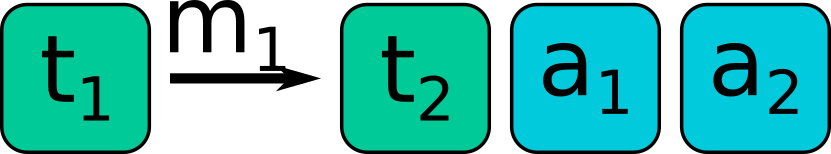
\includegraphics[width=0.7\textwidth]{images/final/domain_example}
\end{figure}
